\documentclass{beamer}

\usepackage[utf8]{inputenc}
\usepackage[T1]{fontenc}
\usepackage[french]{babel}


\usepackage{graphicx}

% Pour inclure des images en .svg
\usepackage{svg}

%Des packages dont je ne me souviens plus trop ce que ça fait
\usepackage{wrapfig} %=> Pas utile je crois
\usepackage{caption} %=> Pas utile je crois
\usepackage{placeins} %=> Pas utile je crois
\usepackage{hyperref} %=> Pour avoir des liens (quand tu cliques sur les titres dans le sommaire)
\usepackage{amssymb,amsmath,mathrsfs, amsthm} %=> Pour les maths, important
\usepackage{multirow} %=> Pour faire des trucs bizarres avec les tableaux

\usepackage{dirtree}

\usepackage{listings}
\usepackage{xcolor}

\lstset{ % General setup for the package
    language=Python,
    basicstyle=\small\sffamily,
    numbers=left,
     numberstyle=\tiny,
    frame=tb,
    tabsize=4,
    columns=fixed,
    showstringspaces=false,
    showtabs=false,
    keepspaces,
    commentstyle=\color{red},
    keywordstyle=\color{blue}
}
\newcommand\nom[2][]{#1~\textsc{#2}}

\title{Rapport de Stage L3\\Mise en place d'un cache Logiciel avec Nix}
\author{Maurice Debray}
\date{}

%Theme beamer, defini l'apparence
\usetheme[block=fill, numbering=fraction]{metropolis}
\setbeamertemplate{section in toc}[sections numbered]
\setbeamertemplate{subsection in toc}[subsections numbered]
%\usecolortheme{crane}
\setbeamertemplate{itemize items}[circle]
\setbeamertemplate{enumerate item}[default]


\setbeamertemplate{navigation symbols}{}


\makeatletter
\setbeamertemplate{section page}{
  \centering
  \begin{minipage}{22em}
    \raggedright
    \usebeamercolor[fg]{section title}
    \usebeamerfont{section title}
    \thesection.~\insertsectionhead\\[-1ex]
    \usebeamertemplate*{progress bar in section page}
    \par
    \ifx\insertsubsectionhead\@empty\else%
      \usebeamercolor[fg]{subsection title}%
      \usebeamerfont{subsection title}%
      \thesubsection.~\insertsubsectionhead
    \fi
  \end{minipage}
  \par
  \vspace{\baselineskip}
}
\makeatother

%\setbeamertemplate{footline}[frame number]{}


\begin{document}
\begin{frame}
  \maketitle
\end{frame}

\begin{frame}{Introduction}
\end{frame}

\begin{frame}{Sommaire}
  \tableofcontents
\end{frame}

\section{Le gestionnaire de paquets \emph{nix}}

\begin{frame}{Propriétés clefs}
	\begin{itemize}
		\item Essaie de réduire complètement les effets de bord lors de la compilation
		\item Spécification fonctionnelle des paquets sans effets de bord autre que la crétion d'instruction de compilation.
	\end{itemize}

\end{frame}

\begin{frame}{Le store de nix}

\begin{itemize}
	\item Une base de donnée sqlite qui stocke les informations \og{}\emph{A dépend de B}\fg{}.
	\item Un répertoire immutable (éditable uniquement par le démon nix)
\end{itemize}

\dirtree{%
.1 /nix/store:.
.2 aaa\dots-prgm:.
.3 linkToDep -> /nix/store/bbb\dots-dep1.
.3 file\_containing\_ref\_to\_dep2.
.2 bbb\dots-dep1.
.2 ccc\dots-dep2.
.2 ddd\dots-other-program.
}

\begin{block}{Propriété (Appliquée par le démon nix)}
	Si la base de donnée contient \og{}\emph{A dépend de B}\fg{} $\Rightarrow$ on ne peut pas supprimer A sans supprimer aussi B
\end{block}
\end{frame}

\begin{frame}{Ajouter une dérivation au store (Réalisation)}
\begin{block}{En compilant à partir d'instructions de compilation}
Fichiers \texttt{.drv} qui spécifie:
\begin{itemize}
	\item \emph{builder} (executable + arguments)
	\item Dépendances
\end{itemize}

Instanciation = \'Execution du \emph{builder} dans une sandbox où seules les dépendances sont accessibles.

\end{block}

\begin{block}{A partir d'une source externe}
Ajoute d'un chemin directement à partir:
\begin{itemize}
	\item d'un cache nixos
	\item d'un fichier local
	\end{itemize}
\end{block}

\end{frame}

\begin{frame}{Le langage \emph{nix} (\'Evaluation)}

	Langage qui permet la spécification de paquets (et dont le principal effet de bord est de créer les fichiers \emph{.drv})

\end{frame}

\begin{frame}{Pourquoi utiliser \emph{nix}}

Avoir une infrasctructure résiliente

\begin{itemize}
	\item Une conservation automatisée:
		\begin{itemize}
			\item des sources
			\item des résultats de compilation
		\end{itemize}
	\item Centralisation des résultats de compilation (cache/dépôt nixos)
	\item Facile de revenir en arrière sur des systèmes entiers avec \emph{NixOS}.
\end{itemize}
\end{frame}

\section{Lister toutes les dépendances}

\begin{frame}{Le système de dépendance de nix}

On a vu: Liens de dépendance forts et assurés par l'immutabilité du store.

\vspace{0.5cm}

\begin{block}{Problématique}
	Comment nix détermine les dépendances d'un \emph{store-path}
\end{block}

\end{frame}

\begin{frame}{Piste 1: Les dépendances sont les dépendances de compilation}

	\begin{itemize}
		\item Simple
		\item On est sûr de rien oublier
	\end{itemize}
	Mais
	\begin{itemize}
		\item On récupère trop de dépendances $\Rightarrow$ Démo
	\end{itemize}

	On ne veut garder que ce qui est nécessaire au runtime.

\end{frame}

\begin{frame}{Piste 2: On ne garde que ce qui est nécessaire au runtime}

	\begin{block}{Heuristique de \emph{nix}}
		Si le hash d'un chemin apparait dans la sérialisation du \emph{store-path} alors il s'agit d'une dépendance au \emph{runtime}.
	\end{block}

	Cette heuristique (en plus d'être très simple) fonctionne très bien en pratique.

	\begin{alert}{Problème}
		On peut aboutir dans un état où re-compiler un paquet est impossible.
	\end{alert}

\end{frame}

\begin{frame}{La clôture étendue}

	Coder une fonction qui crée une dérivation dont les dépendances sont:
	\begin{itemize}
		\item Les fichiers \texttt{.drv}
		\item Les résultats de la réalisation des \texttt{.drv}
		\item Les fichiers de code \emph{nix}
	\end{itemize}

	\vspace{0.3cm}
	Plusieurs façons de le faire mais jamais satisfaisantes.
\end{frame}

\begin{frame}{En examinant l'argument de \texttt{builtins.derivation}}
	Solution utilisée sur plusieurs dépôts mais fausse.
\end{frame}

\begin{frame}{En codant notre propre builtin}
	Trop long \tiny{, mais il existe des PR qui font déjà une partie de travail}
\end{frame}

\begin{frame}{En utilisant un \emph{builtin} bugué}

	Il existe un builtin qui a le comportement souhaité. Cependant ce comportement est causé par un bug: \url{https://github.com/NixOS/nix/issues/7299}

	\begin{center}
		\texttt{exportReferenceGraph = [ pkg ]}
	\end{center}

	\begin{itemize}
		\item Attribut dans le fichier \texttt{.drv} qui demande à mettre à disposition des informations sur un paquet spécifique (dépendances, \dots) lors de la réalisation du \texttt{.drv} contenant cet attribut
		\item Normalement fait pour manipuler la closure \emph{runtime} mais on peut tricher.
	\end{itemize}
\end{frame}


\section{Le cache}

\begin{frame}{Nettoyer le \texttt{nix-store}: le garbage collector}

On veut un mécanisme pour enlever ce qui n'est plus utilisé

\dirtree{%
.1 /nix/store:.
.2 aaa\dots-prgm:.
.3 linkToDep -> /nix/store/bbb\dots-dep1.
.3 file\_containing\_ref\_to\_dep2.
.2 bbb\dots-dep1.
.2 ccc\dots-dep2.
.2 ddd\dots-other-program.
}
\vspace{0.3cm}

\dirtree{%
.1 /nix/var/nix/gcroots:.
.2 gcroots1 -> /nix/store/aaa\dots-prgm.
}

L'execution de \texttt{nix-collect-garbage} enlève uniquement \texttt{ddd\dots-other-program}
\end{frame}

\begin{frame}{Processus de mise en cache}

	\centering
	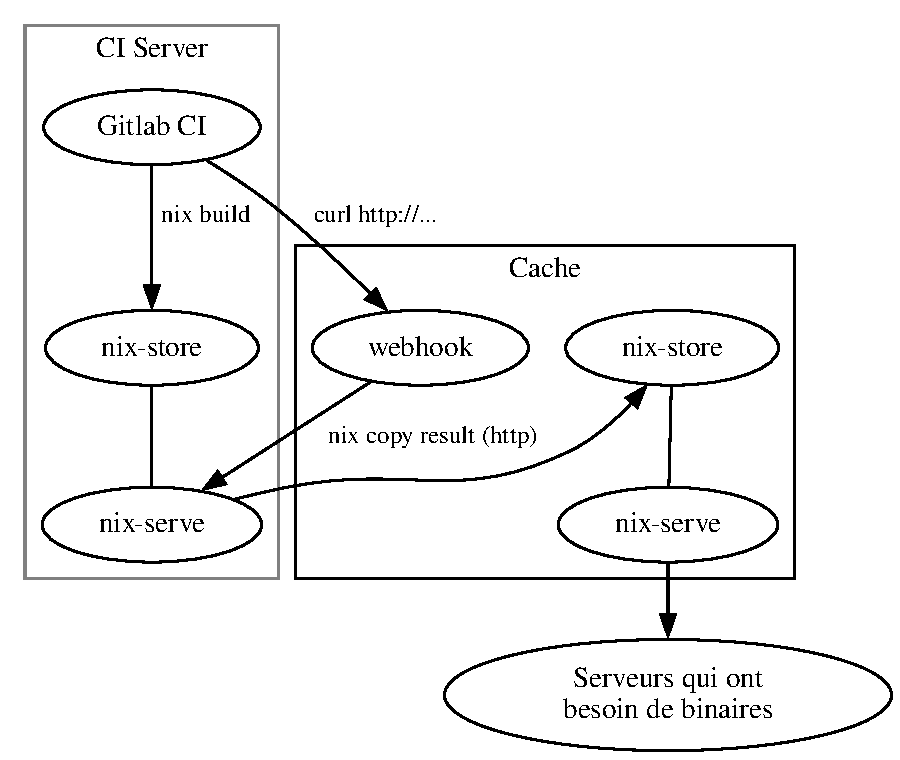
\includegraphics[height=7cm]{../media/ci.pdf}

Architecture du cache
\end{frame}
\begin{frame}{Stockage des gcroots}
\texttt{/nix/var/nix/gcroots/}\\
\texttt{[PATH\_TO\_ORGA]/[REPO]/[BRANCH]/[COMMIT\_HASH]}

\vspace{0.5cm}

	Un outil pour gérer les roots: \texttt{inspect-gcroots}


	Fonctionnalités:

	\begin{itemize}
	\item Suppression des gcroots avec deux politiques de rétention:
		\begin{itemize}
	\item Dates du commit
	\item On garde les $n$ derniers commits (selon la date)
\end{itemize}
	\item Visualisation des commits
	\item Check des dates de commit enregistrées
\end{itemize}
\end{frame}

\section{Conclusion}

\begin{frame}{Conclusion}
	\begin{itemize}
		\item C'est long de documenter son code mais c'est utile
	\end{itemize}

\end{frame}

\end{document}
